\documentclass[a4paper,10pt]{article}

% ============================================================================
% កញ្ចប់បណ្ណាល័យ (Packages)
% ============================================================================
\usepackage[a4paper, left=0.95cm, right=0.95cm, top=1.0cm, bottom=1.1cm, footskip=0.5cm]{geometry}
\usepackage{fontspec}
\usepackage{amsmath, amssymb}
\usepackage{array, longtable, multirow, colortbl}
\usepackage[table]{xcolor}
\usepackage{enumitem}
\usepackage{pifont}
\usepackage{fancyhdr}
\usepackage{tikz}
\usetikzlibrary{calc, arrows.meta, angles, quotes, decorations.markings, babel}

% ============================================================================
% ការកំណត់ពុម្ពអក្សរ (Fonts Configuration)
% ============================================================================
\defaultfontfeatures{Ligatures=TeX}

% Cross-platform font path resolver (Windows local + Linux/Cloud repo fonts/)
\providecommand{\NGSFindFonts}{%
  \IfFileExists{C:/Windows/Fonts/cambria.ttc}{%
    \def\NGSSysPath{C:/Windows/Fonts/}%
    \def\NGSUserPath{C:/Users/KIT/AppData/Local/Microsoft/Windows/Fonts/}%
  }{%
    \IfFileExists{./fonts/KhmerOSsiemreap.ttf}{\def\NGSSysPath{./fonts/}\def\NGSUserPath{./fonts/}}{%
    \IfFileExists{../fonts/KhmerOSsiemreap.ttf}{\def\NGSSysPath{../fonts/}\def\NGSUserPath{../fonts/}}{%
    \IfFileExists{../../fonts/KhmerOSsiemreap.ttf}{\def\NGSSysPath{../../fonts/}\def\NGSUserPath{../../fonts/}}{%
    \IfFileExists{../../../fonts/KhmerOSsiemreap.ttf}{\def\NGSSysPath{../../../fonts/}\def\NGSUserPath{../../../fonts/}}{%
    \IfFileExists{../../../../fonts/KhmerOSsiemreap.ttf}{\def\NGSSysPath{../../../../fonts/}\def\NGSUserPath{../../../../fonts/}}{%
    \IfFileExists{../../../../../fonts/KhmerOSsiemreap.ttf}{\def\NGSSysPath{../../../../../fonts/}\def\NGSUserPath{../../../../../fonts/}}{%
    \IfFileExists{../../../../../../fonts/KhmerOSsiemreap.ttf}{\def\NGSSysPath{../../../../../../fonts/}\def\NGSUserPath{../../../../../../fonts/}}{%
      \def\NGSSysPath{../../../../../../../fonts/}\def\NGSUserPath{../../../../../../../fonts/}%
    }}}}}}}%
  }%
}
\NGSFindFonts

\setmainfont[
  Path={\NGSUserPath},
  Extension=.ttf,
  Script=Khmer,
  BoldFont={KhmerOSsiemreap},
  BoldFeatures={FakeBold=1.8},
  ItalicFont={KhmerOSsiemreap},
  ItalicFeatures={FakeSlant=0.3},
  BoldItalicFont={KhmerOSsiemreap},
  BoldItalicFeatures={FakeBold=1.8, FakeSlant=0.3}
]{KhmerOSsiemreap}

\newfontfamily\muol[
  Path={\NGSUserPath},
  Extension=.ttf,
  Script=Khmer
]{KhmerOSmuollight}

\newfontfamily\NagaBold[
  Path={\NGSUserPath},
  Extension=.ttf
]{AKbalthom Naga Bold}

\newfontfamily\CalibriFont[
  Path={\NGSSysPath},
  Extension=.ttf
]{calibri}

% ============================================================================
% ការកំណត់ពណ៌ និងទម្រង់ទំព័រ (Colors & Page Style)
% ============================================================================
\definecolor{stepgray}{HTML}{D9D9D9}
\definecolor{headgray}{HTML}{F2F2F2}
\definecolor{boxgray}{HTML}{D9D9D9}
\definecolor{darkred}{HTML}{C00000}
\definecolor{red5e}{HTML}{FF0000}
\definecolor{triblue}{HTML}{DAE8FC}
\definecolor{triborders}{HTML}{6C8EBF}
\definecolor{arrowblue}{HTML}{4472C4}

\pagestyle{fancy}
\fancyhf{}
\renewcommand{\headrulewidth}{0pt}
\fancyfoot[R]{\CalibriFont\fontsize{11pt}{13pt}\selectfont\thepage}

\setlength{\parindent}{0pt}
\setlength{\parskip}{0pt}
\setlength{\tabcolsep}{3.8pt}

% ប្រភេទជួរឈរតារាងតម្រឹមឆ្វេង (Left-aligned table column type)
\newcolumntype{L}[1]{>{\raggedright\arraybackslash}p{#1}}

% ============================================================================
% ម៉ាក្រូជំនួយ (Helper Macros)
% ============================================================================
\newcommand{\fiveE}[1]{{\NagaBold\fontsize{9.5pt}{13pt}\selectfont\textcolor{red5e}{#1}}}
\newcommand{\timenote}[1]{\textcolor{darkred}{\textit{#1}}}
\newcommand{\redsub}[1]{\textcolor{darkred}{#1}}
\newcommand{\graybox}[1]{\colorbox{boxgray}{\strut\hspace{2pt}#1\hspace{2pt}}}
\newcommand{\ditem}{\tikz[baseline=-0.5ex]\fill (0,0.42ex) -- (0.42ex,0) -- (0,-0.42ex) -- (-0.42ex,0) -- cycle;\hspace{0.3em}}
\newcommand{\cnum}[1]{{\fontsize{10.5pt}{12pt}\selectfont\ding{\numexpr181+#1\relax}}\hspace{0.2em}}
\newcommand{\cfig}[1]{\par\vspace{2pt}{\centering #1\par}\vspace{2pt}}
\newcommand{\stepheader}[1]{\multicolumn{3}{|c|}{\cellcolor{stepgray}\muol #1} \\* \noalign{\hrule height 0.4pt}}

% ក្បាច់ក្រោមបាវចនា (Tacteing Flourish)
\newcommand{\khmflourish}{%
  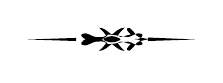
\begin{tikzpicture}[x=0.05bp, y=-0.05bp, baseline=0pt]
    \path[fill=black, nonzero rule]
      (847,-111) .. controls (867,-92) and (921,-137) .. (902,-147)
      .. controls (865,-168) and (826,-126) .. (803,-126)
      .. controls (750,-126) and (704,-146) .. (655,-143)
      .. controls (652,-129) and (616,-116) .. (612,-107)
      .. controls (616,-101) and (651,-89) .. (655,-74)
      .. controls (706,-73) and (747,-92) .. (804,-92)
      .. controls (825,-92) and (871,-48) .. (904,-72)
      .. controls (916,-81) and (866,-126) .. (847,-111)
      (1284,-108) -- (943,-122) -- (943,-97) -- (1284,-108)
      (426,-119) -- (78,-108) -- (426,-97) -- (426,-119)
      (522,-111) .. controls (502,-93) and (446,-136) .. (467,-147)
      .. controls (504,-168) and (543,-126) .. (566,-126)
      .. controls (594,-126) and (619,-118) .. (644,-136)
      .. controls (629,-158) and (612,-176) .. (592,-193)
      .. controls (629,-193) and (655,-163) .. (684,-143)
      .. controls (712,-164) and (739,-193) .. (776,-193)
      .. controls (757,-176) and (740,-157) .. (725,-136)
      .. controls (756,-112) and (783,-141) .. (821,-143)
      .. controls (801,-162) and (774,-192) .. (811,-192)
      .. controls (831,-175) and (849,-156) .. (864,-135)
      .. controls (876,-118) and (943,-114) .. (943,-111)
      .. controls (943,-104) and (876,-101) .. (864,-84)
      .. controls (849,-63) and (831,-44) .. (811,-27)
      .. controls (774,-27) and (801,-57) .. (821,-76)
      .. controls (783,-78) and (756,-107) .. (725,-83)
      .. controls (740,-61) and (757,-43) .. (776,-26)
      .. controls (739,-26) and (712,-55) .. (684,-76)
      .. controls (655,-56) and (629,-26) .. (592,-26)
      .. controls (612,-43) and (629,-61) .. (644,-83)
      .. controls (619,-101) and (594,-92) .. (566,-92)
      .. controls (544,-92) and (498,-48) .. (465,-72)
      .. controls (451,-82) and (502,-129) .. (522,-111)
      (684,-132) .. controls (661,-132) and (623,-115) .. (623,-109)
      .. controls (623,-101) and (663,-87) .. (684,-87)
      .. controls (706,-87) and (746,-101) .. (746,-109)
      .. controls (746,-115) and (708,-132) .. (684,-132)
      (684,-116) .. controls (675,-116) and (659,-112) .. (659,-109)
      .. controls (659,-105) and (676,-102) .. (684,-102)
      .. controls (693,-102) and (710,-105) .. (710,-109)
      .. controls (710,-112) and (694,-116) .. (684,-116);
  \end{tikzpicture}%
}

% ============================================================================
% ម៉ាក្រូគូសរូបធរណីមាត្រ (Reusable TikZ Geometric Macros)
% ============================================================================

% រ៉ាប៉ទ័រ (Protractor centered at (0,0))
\newcommand{\drawProtractor}{%
  \begin{scope}
    \fill[white, fill opacity=0.92] (-1.65,-0.10) -- (1.65,-0.10) -- (1.65,0) arc (0:180:1.65) -- cycle;
    \draw[thin, gray!80!black] (-1.65,-0.10) -- (1.65,-0.10) -- (1.65,0) arc (0:180:1.65) -- cycle;
    \draw[thin, gray!80!black] (1.08,0) arc (0:180:1.08) -- (-1.08,0) -- cycle;
    \draw[thin, gray!80!black] (0.20,0) arc (0:180:0.20);
    \draw[thin, gray!80!black] (0,0) -- (0,0.20);
    % ក្រិតដឺក្រេ (Degree ticks)
    \foreach \a in {0,2,...,180} {
      \draw[very thin, gray!70!black] (\a:1.57) -- (\a:1.65);
    }
    \foreach \a in {0,5,...,180} {
      \draw[very thin, gray!85!black] (\a:1.51) -- (\a:1.65);
      \draw[very thin, gray!85!black] (\a:1.08) -- (\a:1.15);
    }
    \foreach \a in {0,10,...,180} {
      \draw[thin, black!80] (\a:1.43) -- (\a:1.65);
      \draw[thin, black!80] (\a:1.08) -- (\a:1.20);
      \pgfmathtruncatemacro{\inang}{180-\a}
      \pgfmathsetmacro{\lbla}{\a==0 ? 2.8 : (\a==180 ? 177.2 : \a)}
      \node[font=\tiny, scale=0.44] at (\lbla:1.34) {\a};
      \node[font=\tiny, scale=0.40] at (\lbla:0.96) {\inang};
      \ifnum\a>0
        \ifnum\a<180
          \draw[very thin, black!60] (\a:0.32) -- (\a:0.82);
        \fi
      \fi
    }
  \end{scope}
}

% បន្ទាត់ក្រិត (Ruler along angle 50 deg)
\newcommand{\drawRuler}[1][50]{%
  \begin{scope}[rotate=#1]
    \fill[gray!10, draw=black!70, thin] (-0.22,0) rectangle (2.45,-0.30);
    \foreach \i in {0,1,...,30} {
      \draw[very thin, black!60] (\i*0.075,0) -- (\i*0.075,-0.06);
    }
    \foreach \i in {0,1,...,12} {
      \draw[very thin, black!80] (\i*0.1875,0) -- (\i*0.1875,-0.10);
    }
    \foreach \n in {0,1,...,6} {
      \draw[thin, black] (\n*0.375,0) -- (\n*0.375,-0.14);
      \node[font=\tiny, scale=0.46, rotate=#1-90] at (\n*0.375,-0.21) {\n};
    }
  \end{scope}
}

% ខ្មៅដៃ (Small Pencil)
\newcommand{\drawPencil}[2]{%
  \begin{scope}[shift={(#1)}, rotate=#2]
    \draw[fill=gray!60, draw=black, very thin] (0,0) -- (0.055,0.16) -- (-0.055,0.16) -- cycle;
    \fill[black] (0,0) -- (0.02,0.05) -- (-0.02,0.05) -- cycle;
    \draw[fill=gray!35, draw=black, very thin] (-0.055,0.16) rectangle (0.055,0.68);
  \end{scope}
}

% បន្ទាត់ស្របពីរកាត់ដោយខ្នាត់មួយ (Parallel lines cut by exact 60 deg transversal)
\newcommand{\drawParallelBase}{%
  \draw[thin] (-2.15, 0.50) -- (2.15, 0.50) node[right, font=\scriptsize] {$(d_1)$};
  \draw[thin] (-2.15,-0.50) -- (2.15,-0.50) node[right, font=\scriptsize] {$(d_2)$};
  \draw[-{Stealth[scale=0.6]}, thin] (1.15, 0.50) -- (1.30, 0.50);
  \draw[-{Stealth[scale=0.6]}, thin] (1.15,-0.50) -- (1.30,-0.50);
  \coordinate (A) at (0.2887, 0.50);
  \coordinate (B) at (-0.2887,-0.50);
  \draw[thin] (-0.5889,-1.02) -- (0.5889, 1.02) node[above, font=\scriptsize, inner sep=1pt] {$(\Delta)$};
  \fill (A) circle (1.1pt) node[above left, font=\scriptsize, inner sep=1.5pt] {$A$};
  \fill (B) circle (1.1pt) node[below right, font=\scriptsize, inner sep=1.5pt] {$B$};
}

% ត្រីកោណត្រួតគ្នា សម្រាប់លំហាត់ប្រតិបត្តិ (Collinear rays ABD and AEC, AB = AE, AD = AC)
\newcommand{\drawPracticeTriangles}[1][1.0]{%
  \begin{tikzpicture}[scale=#1, every node/.style={font=\scriptsize}]
    \coordinate (A) at (0,0);
    \coordinate (B) at (1.3703, 0.6101);
    \coordinate (E) at (1.3703,-0.6101);
    \coordinate (D) at (2.5123, 1.1185);
    \coordinate (C) at (2.5123,-1.1185);
    \draw[thin] (A) -- (D) -- (E) -- cycle;
    \draw[thin] (A) -- (C) -- (B) -- cycle;
    % គំនូសសម្គាល់ជ្រុងស្មើគ្នា (Perpendicular tick marks on AB and AE)
    \draw[thin] ($(A)!0.52!(B)+(-0.0366,0.0822)$) -- ($(A)!0.52!(B)+(0.0366,-0.0822)$);
    \draw[thin] ($(A)!0.52!(E)+(0.0366,0.0822)$) -- ($(A)!0.52!(E)+(-0.0366,-0.0822)$);
    % គំនូសសម្គាល់មុំស្មើគ្នា (Exact angle arcs at B and E touching both adjacent sides)
    \draw[thin] ($(B)+(204:0.24)$) arc (204:303.45:0.24);
    \draw[thin] ($(E)+(56.55:0.24)$) arc (56.55:156:0.24);
    \node[left] at (A) {$A$};
    \node[above left, inner sep=1.5pt] at (B) {$B$};
    \node[below left, inner sep=1.5pt] at (E) {$E$};
    \node[above right, inner sep=1pt] at (D) {$D$};
    \node[below right, inner sep=1pt] at (C) {$C$};
  \end{tikzpicture}%
}

% ============================================================================
% ចាប់ផ្ដើមឯកសារ (Document Body)
% ============================================================================
\begin{document}
\fontsize{9.5pt}{15.8pt}\selectfont

% -------------------- ក្បាលកិច្ចតែងការ (Header) --------------------
\begin{center}
  {\muol\fontsize{11pt}{16pt}\selectfont ព្រះរាជាណាចក្រកម្ពុជា}\\[2pt]
  {\muol\fontsize{10pt}{15pt}\selectfont ជាតិ សាសនា ព្រះមហាក្សត្រ}\\[1pt]
  \khmflourish
\end{center}

\vspace{-12pt}
{\muol\fontsize{10pt}{15pt}\selectfont អនុវិទ្យាល័យព្រះក្រសាំង}

\vspace{4pt}
\begin{center}
  {\muol\fontsize{10pt}{15pt}\selectfont កិច្ចតែងការបង្រៀន}
\end{center}
\vspace{2pt}

% -------------------- ព័ត៌មានទូទៅ (Metadata) --------------------
{\renewcommand{\arraystretch}{1.10}
\hspace*{4.6cm}%
\begin{tabular}{@{}l l l@{}}
  - \hspace{0.35cm} មុខវិជ្ជា & : & គណិតវិទ្យា ថ្នាក់ទី៨ \\
  - \hspace{0.35cm} ចំណងជើងមេរៀន & : & មេរៀនទី១២ ការប្រៀបធៀបត្រីកោណ \\
  - \hspace{0.35cm} ចំណងជើងរង & : & ១.២. លក្ខខណ្ឌនៃត្រីកោណប៉ុនគ្នា \\
  & & ១.២.១ ជ្រុងមួយប៉ុនគ្នាជាប់និងមុំពីរប៉ុនរៀងគ្នា \\
  - \hspace{0.35cm} រយៈពេល & : & ១ ម៉ោងសិក្សា (៤៥នាទី) \\
  - \hspace{0.35cm} បង្រៀនដោយ & : & ហុក ប៊ុនថែន \\
  - \hspace{0.35cm} កាលបរិច្ឆេទ & : & ០៩ កញ្ញា ២០២៦ \\
\end{tabular}

\vspace{3pt}

% -------------------- I. វត្ថុបំណង --------------------
\textbf{I.} {\muol វត្ថុបំណង}\\[2pt]
\hspace*{0.55cm}%
\begin{tabular}{@{}l l l@{}}
  $\circ$ \hspace{0.25cm} វិជ្ជាសម្បទា & : & សិស្សកំណត់បានពីលក្ខខណ្ឌនៃត្រីកោណពីរប៉ុនគ្នាក្នុងករណី ជ្រុងមួយប៉ុនគ្នាជាប់នឹងមុំពីរប៉ុនរៀងគ្នា (ម.ជ.ម) \\
  & & បានត្រឹមត្រូវ តាមរយៈសកម្មភាពរុករក ការសង្កេត Slide Animation និងការឆ្លើយសំណួរបំផុសរបស់គ្រូ។ \\
  $\circ$ \hspace{0.25cm} បំណិនសម្បទា & : & សិស្សបកស្រាយ និងប្រើប្រាស់ លក្ខខណ្ឌ (ម.ជ.ម) ដើម្បីស្រាយបញ្ជាក់ត្រីកោណពីរប៉ុនគ្នាបានច្បាស់លាស់ \\
  $\circ$ & & តាមរយៈ ការពិភាក្សា និងការធ្វើលំហាត់ប្រតិបត្តិ។ \\
  $\circ$ \hspace{0.25cm} ចរិយាសម្បទា & : & សិស្សមានស្មារតី សហការនិងយកចិត្តទុកដាក់ ក្នុងការដោះស្រាយលំហាត់ដោយការទទួលខុសត្រូវជាប្រចាំ \\
  & & តាមរយៈ ការអនុវត្តផ្ទាល់ជាមួយដៃគូ។ \\
\end{tabular}

\vspace{3pt}

% -------------------- II. សម្ភារៈឧបទេស --------------------
\textbf{II.} {\muol សម្ភារៈឧបទេស}\\[2pt]
\hspace*{0.55cm}$\bullet$ \hspace{0.35cm} សៀវភៅសិក្សាគោលថ្នាក់ទី៨ សន្លឹកកិច្ចការ Slide Animation បន្ទះរូបត្រីកោណ

\vspace{3pt}

% -------------------- III. វិធីសាស្រ្តបង្រៀន --------------------
\textbf{III.} {\muol វិធីសាស្រ្តបង្រៀន}\\[2pt]
\hspace*{0.55cm}%
\begin{tabular}{@{}l l l@{}}
  $\bullet$ \hspace{0.35cm} គោលវិធី & : \hspace{0.7cm} & សិស្សមជ្ឈមណ្ឌល \\
  $\bullet$ \hspace{0.35cm} យុទ្ធវិធីបង្រៀន & : & ស្ថាបនានិយម គម្រូ 5Es \\
\end{tabular}
}

\vspace{3pt}

% -------------------- III. ដំណើរការបង្រៀន --------------------
\textbf{III.} {\muol ដំណើរការបង្រៀន}

\vspace{-3pt}

% ============================================================================
% តារាងដំណើរការបង្រៀន (Modular Multi-Row 3-Column Lesson Plan Table)
% បច្ចេកទេស៖ បំបែកតារាងជាជួរដេកតូចៗតាមផ្នែកនីមួយៗ (ដោយមិនដាក់ \hline នៅចន្លោះជួរតូចៗ)
% និងប្រើ \endhead / \endfoot ដើម្បីឱ្យ LaTeX បំពេញក្រដាសនីមួយៗឱ្យពេញ ១០០% ទើបឆ្លងទំព័រថ្មី។
% ============================================================================
\renewcommand{\arraystretch}{1.18}
\begin{longtable}{|L{5.50cm}|L{7.90cm}|L{4.80cm}|}
\hline
\rowcolor{headgray}
\multicolumn{1}{|c|}{\muol សកម្មភាពគ្រូ} &
\multicolumn{1}{c|}{\muol ខ្លឹមសារមេរៀន} &
\multicolumn{1}{c|}{\muol សកម្មភាពសិស្ស} \\
\hline
\endfirsthead

\hline
\endhead

\hline
\endfoot

\hline
\endlastfoot

% ==================== ជំហានទី១ ====================
\stepheader{ជំហានទី១ (រដ្ឋបាលថ្នាក់)}
- ពិនិត្យអវត្តមាន \newline
- ពិនិត្យអនាម័យ \newline
- ពង្រឹងវិន័យ និងសណ្ដាប់ធ្នាប់
&
\hspace*{0.3cm}- រដ្ឋបាលថ្នាក់ \newline
\hspace*{0.3cm}- អនាម័យថ្នាក់រៀន \newline
\hspace*{0.3cm}- សណ្ដាប់ធ្នាប់ថ្នាក់រៀន
&
- រាយការណ៍ \\
\hline

% ==================== ជំហានទី២ ====================
\stepheader{ជំហានទី២ (កិច្ចការផ្ទះ +ទំនាក់ទំនងមេរៀនថ្មី)}
% --- ផ្នែក 2.1: កំណែកិច្ចការផ្ទះ (ប្រធាន និងរូបភាព) ---
\mbox{- ពិនិត្យកិច្ចការផ្ទះរបស់សិស្សនៅផ្ទះជាមុន} \newline
- សរសើរលើកទឹកចិត្តសិស្សដែលបានខិត\newline
\hspace*{0.2cm}ខំធ្វើកិច្ចការបានល្អ \newline
- បង្ហាញចម្លើយ (Slide) លើក្ដារខៀន \newline
\timenote{ចំណាយពេលឱ្យតិចបំផុតកុំឱ្យលើស 3min}
&
\centerline{\redsub{កំណែកិច្ចការផ្ទះ}}
\hspace*{0.2cm}១. ពន្យល់ថាហេតុអ្វីបានជាត្រីកោណពីរខាងក្រោម \newline
\hspace*{0.5cm}មិនប៉ុនគ្នា?
\cfig{%
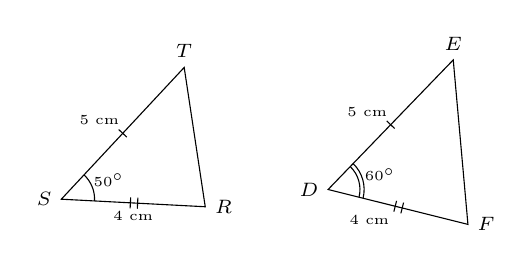
\begin{tikzpicture}[scale=0.88, every node/.style={font=\scriptsize}]
  % ត្រីកោណទី១: STR (ST = 5cm -> 2.60, SR = 4cm -> 2.08, angle S = 50 deg exact)
  \begin{scope}
    \coordinate (S) at (0,0);
    \coordinate (R) at (2.0771,-0.1089);
    \coordinate (T) at (1.7732,1.9015);
    \draw[thin] (S) -- (R) -- (T) -- cycle;
    \draw[thin] ($(S)!0.5!(T)+(137:0.08)$) -- ($(S)!0.5!(T)+(-43:0.08)$);
    \draw[thin] ($(S)!0.48!(R)+(87:0.08)$) -- ($(S)!0.48!(R)+(-93:0.08)$);
    \draw[thin] ($(S)!0.53!(R)+(87:0.08)$) -- ($(S)!0.53!(R)+(-93:0.08)$);
    \draw[thin] (-3:0.48) arc (-3:47:0.48);
    \node[font=\tiny] at (22:0.74) {$50^\circ$};
    \node[left] at (S) {$S$};
    \node[right] at (R) {$R$};
    \node[above] at (T) {$T$};
    \node[above left, font=\tiny, inner sep=2pt] at ($(S)!0.52!(T)$) {$5\text{ cm}$};
    \node[below, font=\tiny, inner sep=3pt] at ($(S)!0.5!(R)$) {$4\text{ cm}$};
  \end{scope}
  % ត្រីកោណទី២: DEF (DE = 5cm -> 2.60, DF = 4cm -> 2.08, angle D = 60 deg exact)
  \begin{scope}[shift={(3.85,0.14)}]
    \coordinate (D) at (0,0);
    \coordinate (F) at (2.0182,-0.5032);
    \coordinate (E) at (1.8061,1.8703);
    \draw[thin] (D) -- (F) -- (E) -- cycle;
    \draw[thin] ($(D)!0.5!(E)+(136:0.08)$) -- ($(D)!0.5!(E)+(-44:0.08)$);
    \draw[thin] ($(D)!0.48!(F)+(76:0.08)$) -- ($(D)!0.48!(F)+(-104:0.08)$);
    \draw[thin] ($(D)!0.53!(F)+(76:0.08)$) -- ($(D)!0.53!(F)+(-104:0.08)$);
    \draw[thin] ($(D)+(-14:0.46)$) arc (-14:46:0.46);
    \draw[thin] ($(D)+(-14:0.52)$) arc (-14:46:0.52);
    \node[font=\tiny] at (16:0.78) {$60^\circ$};
    \node[left] at (D) {$D$};
    \node[right] at (F) {$F$};
    \node[above] at (E) {$E$};
    \node[above left, font=\tiny, inner sep=2pt] at ($(D)!0.52!(E)$) {$5\text{ cm}$};
    \node[below left, font=\tiny, inner sep=3pt] at ($(D)!0.50!(F)$) {$4\text{ cm}$};
  \end{scope}
\end{tikzpicture}%
}
&
- សង្កេត និងលើកជាសំណួរបើមាន \\[-2pt]

% --- ផ្នែក 2.2: ចម្លើយកំណែកិច្ចការផ្ទះ (ផ្នែកទី១) ---
&
\centerline{\underline{ចម្លើយ}}
\hspace*{0.2cm}ត្រីកោណពីរប៉ុនគ្នាលុះត្រាតែធាតុត្រូវជាគ្នា ជាធាតុប៉ុនគ្នា \newline
\hspace*{0.2cm}ក្នុង $\Delta STD$ និង $\Delta DEF$ មានធាតុត្រូវគ្នា \newline
\hspace*{0.3cm}$ST = DE = 5\text{cm}$ \hspace{0.15cm} (ធាតុត្រូវគ្នាប៉ុនគ្នា)
&
\par\vspace*{1.1cm}
- ផ្ទៀងផ្ទាត់ចម្លើយ \\

% --- ផ្នែក 2.3: ចម្លើយកំណែកិច្ចការផ្ទះ (ផ្នែកទី២) ---
- ពន្យល់បន្ថែមគំនិតភ័ន្តច្រឡំរបស់សិស្ស \newline
\hspace*{0.2cm}ដែលមានក្នុងពេលធ្វើកិច្ចការផ្ទះ
&
\hspace*{0.3cm}$SR = DF = 4\text{cm}$ \hspace{0.15cm} (ធាតុត្រូវគ្នាប៉ុនគ្នា) \newline
\hspace*{0.3cm}$\angle S = 40^\circ \neq \angle D = 60^\circ$ (ធាតុត្រូវគ្នាមិនប៉ុនគ្នា) \newline
\hspace*{0.1cm}ដូចនេះ \hspace{0.15cm} \graybox{$\Delta STD$ មិនប៉ុន $\Delta DEF$ \hspace{0.1cm} ព្រោះ $\angle S \neq \angle D$}
&
\\[-2pt]

% --- ផ្នែក 2.4: រំលឹកមេរៀនទាក់ទងមេរៀនថ្មី (រ៉ាប៉ទ័រ ជំហានទី១) ---
\par\vspace*{0.3cm}
- រំលឹកពីរបៀបសង់មុំដោយប្រើរាប់ប៉ទ័រ \newline
\timenote{ចំណាយពេលឱ្យតិចបំផុតកុំឱ្យលើស 1.5min}
&
\centerline{\redsub{រំលឹកមេរៀនទាក់ទងមេរៀនថ្មី}}
\hspace*{0.1cm}- របៀបប្រើប្រាស់រ៉ាប៉ទ័រ (\graybox{\textit{Slide Animation}}) \newline
\hspace*{0.3cm}\ditem ជំហានទី១
\cfig{%
\begin{tikzpicture}[scale=0.95]
  \draw[-{Stealth[scale=0.8]}, thin] (0,0) -- (3.2,0);
  \fill (0,0) circle (1.2pt) node[below left, font=\scriptsize] {$O$};
  \fill (2.9,0) circle (1.2pt) node[below, font=\scriptsize] {$A$};
\end{tikzpicture}%
}
&
\par\vspace*{0.3cm}
- សង្កេត និងសាកល្បងគូសតាម \\[-3pt]

% --- ផ្នែក 2.4b: រ៉ាប៉ទ័រ ជំហានទី២ ---
&
\hspace*{0.3cm}\ditem ជំហានទី២
\cfig{%
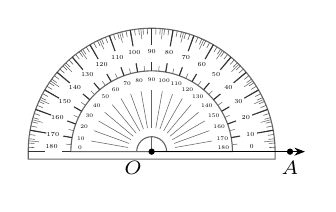
\begin{tikzpicture}[scale=0.95]
  \drawProtractor
  \draw[-{Stealth[scale=0.8]}, thin] (0,0) -- (2.05,0);
  \fill (0,0) circle (1.2pt) node[below left, font=\scriptsize] {$O$};
  \fill (1.85,0) circle (1.2pt) node[below, font=\scriptsize] {$A$};
\end{tikzpicture}%
}
&
\\[-3pt]

% --- ផ្នែក 2.5a: រ៉ាប៉ទ័រ ជំហានទី៣ ---
&
\hspace*{0.2cm}\ditem ជំហានទី៣
\cfig{%
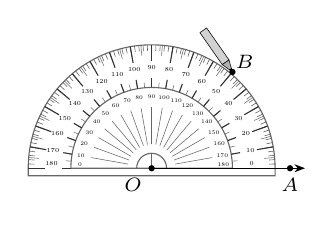
\begin{tikzpicture}[scale=0.95]
  \drawProtractor
  \draw[-{Stealth[scale=0.8]}, thin] (0,0) -- (2.05,0);
  \fill (0,0) circle (1.2pt) node[below left, font=\scriptsize] {$O$};
  \fill (1.85,0) circle (1.2pt) node[below, font=\scriptsize] {$A$};
  \fill (50:1.68) circle (1.2pt) node[above right, font=\scriptsize, inner sep=1pt] {$B$};
  \drawPencil{50:1.68}{35}
\end{tikzpicture}%
}
&
\\[-3pt]

% --- ផ្នែក 2.5b: រ៉ាប៉ទ័រ ជំហានទី៤ ---
&
\hspace*{0.2cm}\ditem ជំហានទី៤
\cfig{%
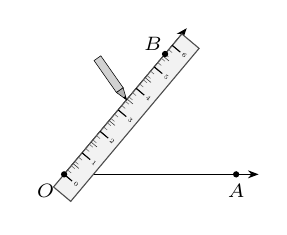
\begin{tikzpicture}[scale=0.95]
  \draw[-{Stealth[scale=0.8]}, thin] (0,0) -- (2.6,0);
  \draw[-{Stealth[scale=0.8]}, thin] (0,0) -- (50:2.55);
  \drawRuler[50]
  \fill (0,0) circle (1.2pt) node[below left, font=\scriptsize] {$O$};
  \fill (2.3,0) circle (1.2pt) node[below, font=\scriptsize] {$A$};
  \fill (50:2.1) circle (1.2pt) node[above left, font=\scriptsize, inner sep=1pt] {$B$};
  \drawPencil{50:1.30}{35}
\end{tikzpicture}%
}
&
\\[-3pt]

% --- ផ្នែក 2.6: រ៉ាប៉ទ័រ ជំហានទី៥ ---
&
\hspace*{0.1cm}\ditem ជំហានទី៥
\cfig{%
\begin{tikzpicture}[scale=0.95]
  \draw[-{Stealth[scale=0.8]}, thin] (0,0) -- (2.7,0);
  \draw[-{Stealth[scale=0.8]}, thin] (0,0) -- (50:2.65);
  \draw[thin, gray!80!black] (0.62,0) arc (0:50:0.62);
  \node[font=\scriptsize] at (25:0.88) {$50^\circ$};
  \fill (0,0) circle (1.2pt) node[below left, font=\scriptsize] {$O$};
  \fill (2.4,0) circle (1.2pt) node[below, font=\scriptsize] {$A$};
  \fill (50:2.15) circle (1.2pt) node[above left, font=\scriptsize] {$B$};
\end{tikzpicture}%
}
&
\par\vspace*{1.2cm}
- សង្កេត និងកត់ចំណាំ \\[-3pt]

% --- ផ្នែក 2.7: ទីតាំង និងលក្ខណៈមុំឆ្លាស់ក្នុង (សង់បន្ទាត់ស្រប) ---
- រំលឹកពីទីតាំង និងលក្ខណៈមុំឆ្លាស់ក្នុង \newline
\timenote{ចំណាយពេលឱ្យតិចបំផុតកុំឱ្យលើស 1.5min} \newline
\mbox{+ សង់បន្ទាត់ស្របពីរកាត់ដោយខ្នាត់មួយ}
&
\hspace*{0.1cm}- ទីតាំង និងលក្ខណៈមុំឆ្លាស់ក្នុង (\graybox{\textit{Slide Animation}})
\cfig{%
\begin{tikzpicture}[scale=0.92]
  \drawParallelBase
\end{tikzpicture}%
}
&
\par\vspace*{0.8cm}
- សង្កេត និងកត់ចំណាំ \\[-3pt]

% --- ផ្នែក 2.8a: កំណត់ទីតាំងមុំឆ្លាស់ក្នុងគូទី១ ---
\par\vspace*{0.5cm}
\mbox{+ កំណត់ទីតាំងមុំឆ្លាស់ក្នុងទាំងពីរគូ}
&
\cfig{%
\begin{tikzpicture}[scale=0.90]
  \drawParallelBase
  \draw[thin] ($(A)+(180:0.32)$) arc (180:240:0.32);
  \node[font=\tiny] at ($(A)+(210:0.20)$) {$1$};
  \draw[thin] ($(B)+(0:0.32)$) arc (0:60:0.32);
  \node[font=\tiny] at ($(B)+(30:0.20)$) {$1$};
  \node[font=\scriptsize] (L1) at (-1.45, 0.14) {មុំឆ្លាស់ក្នុង};
  \draw[-{Stealth[scale=0.6]}, very thin, gray!70!black] (L1.east) to[bend right=15] ($(A)+(215:0.34)$);
  \node[font=\scriptsize] (R1) at (1.45,-0.14) {មុំឆ្លាស់ក្នុង};
  \draw[-{Stealth[scale=0.6]}, very thin, gray!70!black] (R1.west) to[bend right=15] ($(B)+(35:0.34)$);
\end{tikzpicture}%
}
&
\\[-3pt]

% --- ផ្នែក 2.8b: កំណត់ទីតាំងមុំឆ្លាស់ក្នុងគូទី២ ---
&
\cfig{%
\begin{tikzpicture}[scale=0.90]
  \drawParallelBase
  \draw[thin] ($(A)+(-120:0.32)$) arc (-120:0:0.32);
  \node[font=\tiny] at ($(A)+(-60:0.21)$) {$2$};
  \draw[thin] ($(B)+(60:0.32)$) arc (60:180:0.32);
  \node[font=\tiny] at ($(B)+(120:0.21)$) {$2$};
  \node[font=\scriptsize] (R2) at (1.46, 0.14) {មុំឆ្លាស់ក្នុង};
  \draw[-{Stealth[scale=0.6]}, very thin, gray!70!black] (R2.west) to[bend left=12] ($(A)+(-45:0.34)$);
  \node[font=\scriptsize] (L2) at (-1.46,-0.14) {មុំឆ្លាស់ក្នុង};
  \draw[-{Stealth[scale=0.6]}, very thin, gray!70!black] (L2.east) to[bend left=12] ($(B)+(135:0.34)$);
\end{tikzpicture}%
}
&
\\[-3pt]

% --- ផ្នែក 2.9a: សួរអំពីលក្ខណៈរបស់មុំឆ្លាស់ក្នុង (60°) ---
\mbox{+ សួរអំពីលក្ខណៈរបស់មុំឆ្លាស់ក្នុង}
&
\cfig{%
\begin{tikzpicture}[scale=0.86]
  \drawParallelBase
  \draw[thin] ($(A)+(180:0.34)$) arc (180:240:0.34);
  \node[font=\tiny, scale=0.80] at ($(A)+(205:0.52)$) {$60^\circ$};
  \draw[thin] ($(B)+(0:0.34)$) arc (0:60:0.34);
  \node[font=\tiny, scale=0.80] at ($(B)+(25:0.52)$) {$60^\circ$};
  \node[font=\scriptsize] (L1) at (-1.45, 0.10) {មុំឆ្លាស់ក្នុង};
  \draw[-{Stealth[scale=0.6]}, very thin, gray!70!black] (L1.east) to[bend right=18] ($(A)+(225:0.36)$);
  \node[font=\scriptsize] (R1) at (1.45,-0.10) {មុំឆ្លាស់ក្នុង};
  \draw[-{Stealth[scale=0.6]}, very thin, gray!70!black] (R1.west) to[bend right=18] ($(B)+(45:0.36)$);
  \node[font=\scriptsize] at (1.25,-0.88) {$\widehat{A}_1 = \widehat{B}_1 = 60^\circ$};
\end{tikzpicture}%
}
&
- មុំឆ្លាស់ក្នុងមានរង្វាស់ប៉ុនគ្នា \\[-3pt]

% --- ផ្នែក 2.9b: លក្ខណៈរបស់មុំឆ្លាស់ក្នុង (120°) ---
&
\cfig{%
\begin{tikzpicture}[scale=0.86]
  \drawParallelBase
  \draw[thin] ($(A)+(-120:0.34)$) arc (-120:0:0.34);
  \node[font=\tiny, scale=0.80] at ($(A)+(-82:0.45)$) {$120^\circ$};
  \draw[thin] ($(B)+(60:0.34)$) arc (60:180:0.34);
  \node[font=\tiny, scale=0.80] at ($(B)+(98:0.45)$) {$120^\circ$};
  \node[font=\scriptsize] (R2) at (1.46, 0.14) {មុំឆ្លាស់ក្នុង};
  \draw[-{Stealth[scale=0.6]}, very thin, gray!70!black] (R2.west) to[bend left=12] ($(A)+(-32:0.36)$);
  \node[font=\scriptsize] (L2) at (-1.46,-0.14) {មុំឆ្លាស់ក្នុង};
  \draw[-{Stealth[scale=0.6]}, very thin, gray!70!black] (L2.east) to[bend left=12] ($(B)+(148:0.36)$);
  \node[font=\scriptsize] at (1.25,-0.88) {$\widehat{A}_2 = \widehat{B}_2 = 120^\circ$};
\end{tikzpicture}%
}
&
\\[-3pt]

% --- ផ្នែក 2.10: E1 - Engage ---
\fiveE{E1- Engage (3min)} \newline
\mbox{- តើយើងត្រូវស្គាល់ធាតុប៉ុន្មាននៃត្រីកោណពីរ} \newline
\hspace*{0.2cm}\mbox{ទើបអាចសន្និដ្ឋានបានថាត្រីកោណទាំងពីរ} \newline
\hspace*{0.2cm}នោះប៉ុនគ្នា? \newline
\mbox{- ក្នុងត្រីកោណ ABC មួយចំពោះជ្រុង AB} \newline
\hspace*{0.2cm}\mbox{តើមុំណាខ្លះដែលនៅចុងសងខាង និងជាប់} \newline
\hspace*{0.2cm}ជាមួយនឹងជ្រុង AB នេះ?
\par\vspace*{0.15cm}
\mbox{- ប្រសិនបើយើងមិនស្គាល់ធាតុត្រូវគ្នាទាំង៦ទេ} \newline
\hspace*{0.2cm}\mbox{តែយើងអាចស្គាល់ធាតុត្រូវគ្នាចំនួន៣ គូ។} \newline
\hspace*{0.2cm}\mbox{តើយើងអាចថាត្រីកោណពីរនោះប៉ុនគ្នាឬទេ?}
&
\hspace*{0.1cm}- រំលឹកនិយមនន័យត្រីកោណប៉ុនគ្នា
\cfig{%
\begin{tikzpicture}[scale=0.88, every node/.style={font=\scriptsize}]
  \coordinate (A) at (-1.5,0);
  \coordinate (B) at (1.5,0);
  \coordinate (C) at (0,1.68);
  \draw[thin, gray!80!black] (A) -- (B) -- (C) -- cycle;
  \draw[thin, gray!80!black] ($(A)+(0:0.46)$) arc (0:48.24:0.46);
  \node[font=\tiny, scale=0.85] at ($(A)+(24:0.62)$) {$\widehat{A}$};
  \draw[thin, gray!80!black] ($(B)+(131.76:0.46)$) arc (131.76:180:0.46);
  \node[font=\tiny, scale=0.85] at ($(B)+(156:0.62)$) {$\widehat{B}$};
  \draw[thin, gray!80!black] ($(C)+(-131.76:0.38)$) arc (-131.76:-48.24:0.38);
  \node[below left] at (A) {$A$};
  \node[below right] at (B) {$B$};
  \node[above] at (C) {$C$};
  \node[align=center, font=\tiny] (LA) at (-2.75,0.28) {មុំ $\widehat{A}$\\(មុំជាប់ជ្រុង $AB$)};
  \draw[-{Stealth[scale=0.6]}, very thin, gray!70!black] (LA.east) to[bend left=15] ($(A)+(24:0.48)$);
  \node[align=center, font=\tiny] (LB) at (2.75,0.28) {មុំ $\widehat{B}$\\(មុំជាប់ជ្រុង $AB$)};
  \draw[-{Stealth[scale=0.6]}, very thin, gray!70!black] (LB.west) to[bend right=15] ($(B)+(156:0.48)$);
  \node[font=\tiny] (LC) at (1.75,1.55) {មុំ $\widehat{C}$ (មុំឈមនឹងជ្រុង $AB$)};
  \draw[-{Stealth[scale=0.6]}, very thin, gray!70!black] (LC.west) to[bend left=12] ($(C)+(-90:0.40)$);
  \draw[dashed, red!70!black, very thin] (-1.5,0) -- (-1.5,-0.22) -- (1.5,-0.22) -- (1.5,0);
  \node[font=\scriptsize] at (0,-0.38) {ជ្រុង $AB$};
\end{tikzpicture}%
}
\hspace*{0.1cm}- ទាញចំណាប់អារម្មណ៍សិស្សចូលមេរៀនថ្មី
&
\par\vspace*{0.2cm}
- លុះត្រាតែស្គាល់ធាតុត្រូវគ្នាទាំង៦ គូ \newline
\hspace*{0.2cm}ជាធាតុប៉ុនគ្នា
\par\vspace*{0.3cm}
- មុំដែលនៅសងខាងនិងជាប់ជ្រុង AB \newline
\hspace*{0.2cm}គឺ $\angle A$ និង $\angle B$
\par\vspace*{0.8cm}
\mbox{- ចង់ដឹងចម្លើយនិងត្រៀមរៀនមេរៀនថ្មី} \\
\hline

% ==================== ជំហានទី៣ ====================
\stepheader{ជំហានទី៣ (ខ្លឹមសារមេរៀនថ្មី)}
% --- ផ្នែក 3.1: ចំណងជើងមេរៀន និងសំណួរបំផុស E2 ---
\mbox{- សរសេរចំណងជើងមេរៀនថ្មីលើក្ដារខៀន}
\par\vspace*{0.15cm}
\fiveE{E2 - Explore (8min)}
\par\vspace*{0.15cm}
\ditem បញ្ចាំងសំណួរធំៗលើក្ដារខៀន
&
មេរៀនទី១២ \hspace{0.15cm} {\muol ការប្រៀបធៀបត្រីកោណ (ត)} \newline
១.២. លក្ខខណ្ឌនៃត្រីកោណប៉ុនគ្នា \newline
១.២.១ ជ្រុងមួយប៉ុនគ្នាជាប់និងមុំពីរប៉ុនរៀងគ្នា (ម.ជ.ម)
\par\vspace*{0.15cm}
\hspace*{0.2cm}ប្រសិនបើយើងសង់ ត្រីកោណពីរ ដោយស្គាល់ប្រវែងជ្រុង \newline
\hspace*{0.2cm}មួយប៉ុនគ្នា និងមុំពីរនៅចុងសងខាងជ្រុងនោះប៉ុនរៀងគ្នា \newline
\hspace*{0.2cm}តើត្រីកោណទាំងពីរនោះប៉ុនគ្នាដែរឬទេ?
&
- កត់ត្រាចំណងជើងមេរៀន
\par\vspace*{0.8cm}
\ditem ឆ្លើយតាមការយល់ឃើញ \\[-2pt]

% --- ផ្នែក 3.2a: សកម្មភាពរុករក E2 និងរូបត្រីកោណពីរដាច់គ្នា ---
\ditem ចែកសន្លឹកកិច្ចការដែលមានគូសអង្កត់ \newline
\hspace*{0.2cm}$AB = 4\text{cm}$ និងមានកំណត់រង្វាស់មុំ \newline
\hspace*{0.15cm}$\angle A = 45^\circ$ និង $\angle B = 50^\circ$ រួចស្រេច \newline
\hspace*{0.15cm}\mbox{បន្ទាប់មកឱ្យសិស្សប្រើរ៉ាប់ទ័រដើម្បីវាស់មុំ} \newline
\hspace*{0.15cm}និងសង់ត្រីកោណ $ABC$ ។ \newline
\ditem ចែករូបត្រីកោណ A'B'C' ដែលបានសង់ \newline
\hspace*{0.2cm}និងកាត់រួចដែលមានធាតុត្រូវគ្នា ម.ជ.ម \newline
\hspace*{0.2cm}ប៉ុនគ្នាឱ្យសិស្សយកដាក់ត្រួតលើគ្នា
&
\cfig{%
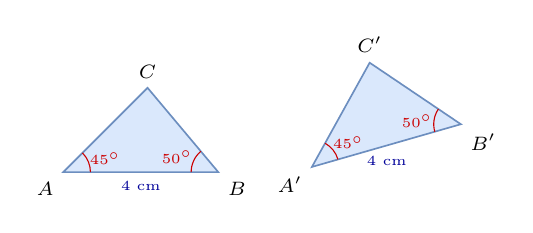
\begin{tikzpicture}[scale=0.82, every node/.style={font=\scriptsize}]
  % ត្រីកោណទី១: ABC (AB = 2.40, exact angles 45 and 50 -> C=(1.3050, 1.3050))
  \begin{scope}[shift={(-2.60,0)}]
    \coordinate (A) at (0,0);
    \coordinate (B) at (2.40,0);
    \coordinate (C) at (1.3050,1.3050);
    \fill[triblue] (A) -- (B) -- (C) -- cycle;
    \draw[triborders, semithick] (A) -- (B) -- (C) -- cycle;
    \draw[red!80!black, thin] (0.42,0) arc (0:45:0.42);
    \node[red!80!black, font=\tiny] at (18:0.68) {$45^\circ$};
    \draw[red!80!black, thin] (1.98,0) arc (180:130:0.42);
    \node[red!80!black, font=\tiny] at ($(B)+(160:0.68)$) {$50^\circ$};
    \node[below left] at (A) {$A$};
    \node[below right] at (B) {$B$};
    \node[above] at (C) {$C$};
    \node[below, blue!60!black, font=\tiny] at (1.20,0) {$4\text{ cm}$};
  \end{scope}
  % ត្រីកោណទី២: A'B'C' (identical congruent triangle, rotated 16 deg, well separated)
  \begin{scope}[shift={(1.25,0.08)}, rotate=16]
    \coordinate (Ap) at (0,0);
    \coordinate (Bp) at (2.40,0);
    \coordinate (Cp) at (1.3050,1.3050);
    \fill[triblue] (Ap) -- (Bp) -- (Cp) -- cycle;
    \draw[triborders, semithick] (Ap) -- (Bp) -- (Cp) -- cycle;
    \draw[red!80!black, thin] (0.42,0) arc (0:45:0.42);
    \node[red!80!black, font=\tiny] at (18:0.68) {$45^\circ$};
    \draw[red!80!black, thin] (1.98,0) arc (180:130:0.42);
    \node[red!80!black, font=\tiny] at ($(Bp)+(160:0.68)$) {$50^\circ$};
    \node[below left] at (Ap) {$A'$};
    \node[below right] at (Bp) {$B'$};
    \node[above] at (Cp) {$C'$};
    \node[below, blue!60!black, font=\tiny] at (1.20,-0.02) {$4\text{ cm}$};
  \end{scope}
\end{tikzpicture}%
}
&
\ditem សង់រូបត្រីកោណ $\Delta ABC$ ជាក្រុមតូច
\par\vspace*{0.15cm}
\ditem យកបន្ទះរូបត្រីកោណ $\Delta A'B'C'$ \newline
ដែលកាត់រួចស្រេច មកដាក់ត្រួតលើ \newline
$\Delta ABC$ ដែលទើបសង់រួច សង្កេតឃើញ \newline
ត្រួតស៊ីគ្នាយ៉ាងល្អ រួចសន្និដ្ឋានថា ត្រី\newline
កោណទាំងពីរជាត្រីកោណប៉ុនគ្នា។ \\[-3pt]

% --- ផ្នែក 3.2b: រូបត្រីកោណត្រួតស៊ីគ្នា និង E3 Explain ---
\ditem នៅពេលយក $\Delta A'B'C'$ មកត្រួតលើ \newline
\hspace*{0.2cm}$\Delta ABC$ តើប្អូនៗសង្កេតឃើញដូចម្ដេច? \newline
\fiveE{E3 - Explain (5min)} \newline
\ditem ប្រើប្រាស់ Slide Animation នៃការសង់ \newline
\hspace*{0.2cm}រូប និងការរំកិលរូបភាពដើម្បីពន្យល់សិស្ស
&
\cfig{%
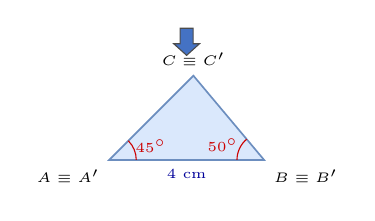
\begin{tikzpicture}[scale=0.82, every node/.style={font=\scriptsize}]
  % សញ្ញាព្រួញចុះក្រោម (centered above superposed congruent triangle)
  \draw[fill=arrowblue, draw=black!70, thin]
    (-0.10,2.04) -- (0.10,2.04) -- (0.10,1.80) -- (0.20,1.80) -- (0.00,1.62) -- (-0.20,1.80) -- (-0.10,1.80) -- cycle;
  % ត្រីកោណត្រួតស៊ីគ្នា: A=A', B=B', C=C' (exact same 2.40 base & 45/50 deg angles)
  \begin{scope}[shift={(-1.20,0)}]
    \coordinate (A2) at (0,0);
    \coordinate (B2) at (2.40,0);
    \coordinate (C2) at (1.3050,1.3050);
    \fill[triblue] (A2) -- (B2) -- (C2) -- cycle;
    \draw[triborders, semithick] (A2) -- (B2) -- (C2) -- cycle;
    \draw[red!80!black, thin] (0.42,0) arc (0:45:0.42);
    \node[red!80!black, font=\tiny] at (18:0.68) {$45^\circ$};
    \draw[red!80!black, thin] (1.98,0) arc (180:130:0.42);
    \node[red!80!black, font=\tiny] at ($(B2)+(160:0.68)$) {$50^\circ$};
    \node[below left, font=\tiny] at (A2) {$A \equiv A'$};
    \node[below right, font=\tiny] at (B2) {$B \equiv B'$};
    \node[above, font=\tiny] at (C2) {$C \equiv C'$};
    \node[below, blue!60!black, font=\tiny] at (1.20,0) {$4\text{ cm}$};
  \end{scope}
\end{tikzpicture}%
}
&
\ditem ឃើញថា ត្រីកោណទាំងពីរត្រួតស៊ីគ្នា \newline
(គ្រប់កំពូល និងជ្រុង ត្រួតស៊ីគ្នា) \newline
\ditem សង្កេត Slide Animation, ឆ្លើយ \newline
សំណួរបំផុស, ទាញទ្រឹស្ដីបទនិងវិបាក \\[-3pt]

% --- ផ្នែក 3.2c: ទ្រឹស្ដីបទ ---
\mbox{\cnum{1}តើយើងអាចទាញជាទ្រឹស្ដីបទរួមដូចម្តេច?}
&
\textbf{ទ្រឹស្ដីបទ :} ត្រីកោណពីរប៉ុនគ្នាកាលណាវាមានជ្រុងមួយ \newline
\hspace*{1.35cm}ប៉ុនគ្នាជាប់នឹងមុំពីរប៉ុនរៀងគ្នា។
&
\ditem ត្រីកោណពីរជាត្រីកោណប៉ុនគ្នា កាល\newline
ណាវាមានជ្រុងមួយប៉ុនគ្នា និងមុំពីរនៅ\newline
ចុងសងខាងនៃជ្រុងនោះប៉ុនរៀងគ្នា \\[-2pt]

% --- ផ្នែក 3.3: វិបាក និងតារាងសង្ខេប ---
\mbox{\cnum{2}នៅពេលដែល $\Delta ABC \cong \Delta A'B'C'$ តាម} \newline
\hspace*{0.2cm}រួចហើយតើធាតុ ៣ ទៀតដែលនៅសល់ \newline
\hspace*{0.2cm}(ជ្រុង២ និងមុំ១) មានលក្ខណៈដូចម្តេច?
&
\cfig{%
\footnotesize
\renewcommand{\arraystretch}{1.12}
\begin{tabular}{|c|c|c|}
  \hline
  សមតិកម្ម & សន្និដ្ឋាន & វិបាក \\
  \hline
  $\angle A = \angle A'$ & & $AC = A'C'$ \\
  $AB = A'B'$ & $\triangle ABC \equiv \triangle A'B'C'$ & $BC = B'C'$ \\
  $\angle B = \angle B'$ & {\tiny (តាមលក្ខខណ្ឌ ម.ជ.ម)} & $\angle C = \angle C'$ \\
  \hline
\end{tabular}%
}
&
\ditem ធាតុដែលនៅសល់ត្រូវតែប៉ុនគ្នាដែរ \newline
($AC = A'C', BC = B'C', \angle C = \angle C'$ \newline
ដែលហៅថា \textbf{វិបាក} \\
\hline

% ==================== ជំហានទី៤ ====================
\stepheader{ជំហានទី៤ (ពង្រីកចំណេះដឹង)}
% --- ផ្នែក 4.1: E4 - Elaborate (លំហាត់គំរូ និងរូបភាព) ---
\fiveE{E4 - Elaborate (10min)} \newline
\ditem ដាក់លំហាត់គំរូ និងសួរសិស្ស \newline
\hspace*{0.25cm}- តើប្រធានបានប្រាប់អ្វីខ្លះ? \newline
\hspace*{0.15cm}- តើជ្រុងណាខ្លះជាជ្រុងត្រូវគ្នា?
\par\vspace*{0.15cm}
\hspace*{0.15cm}- តើមុំណាខ្លះជាមុំត្រូវគ្នា?
&
{\muol លំហាត់គំរូ} \textbf{:} គេឱ្យអង្កត់ $AB$ និង $CD$ ប្រសព្វគ្នាត្រង់ \newline
\hspace*{0.1cm}ចំណុច $E$ ដែល $EA = EB$ និងអង្កត់ $AD$ ស្របនឹងអង្កត់ \newline
\hspace*{0.1cm}$CB$ ។ \newline
\hspace*{0.25cm}ក. ប្រៀបធៀបត្រីកោណ $AED$ និង $BEC$ ។ \newline
\hspace*{0.25cm}ខ. ទាញបញ្ជាក់ថា $ED = EC$ ។
\cfig{%
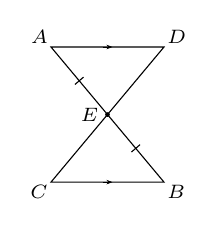
\begin{tikzpicture}[scale=0.78, every node/.style={font=\scriptsize}]
  \coordinate (E) at (0,0);
  \coordinate (A) at (-0.92, 1.10);
  \coordinate (B) at (0.92,-1.10);
  \coordinate (D) at (0.92, 1.10);
  \coordinate (C) at (-0.92,-1.10);
  \draw[thin] (A) -- (D) -- (C) -- (B) -- cycle;
  \draw[-{Stealth[scale=0.55]}, very thin] (-0.08, 1.10) -- (0.08, 1.10);
  \draw[-{Stealth[scale=0.55]}, very thin] (-0.08,-1.10) -- (0.08,-1.10);
  \draw[thin] ($(E)!0.5!(A)+(-0.07,-0.06)$) -- ($(E)!0.5!(A)+(0.07,0.06)$);
  \draw[thin] ($(E)!0.5!(B)+(-0.07,-0.06)$) -- ($(E)!0.5!(B)+(0.07,0.06)$);
  \fill (E) circle (1.1pt) node[left, inner sep=3.2pt] {$E$};
  \node[above left, inner sep=1pt] at (A) {$A$};
  \node[above right, inner sep=1pt] at (D) {$D$};
  \node[below left, inner sep=1pt] at (C) {$C$};
  \node[below right, inner sep=1pt] at (B) {$B$};
\end{tikzpicture}%
}
&
\par\vspace*{0.15cm}
\ditem អានប្រធានលំហាត់ និងឆ្លើយ \newline
- សម្មតិកម្ម : $EA = EB \ , \ AD \parallel CB$ \newline
- ជ្រុងត្រូវគ្នាមាន $EA$ ត្រូវនឹង $EB$ \newline
\hspace*{0.1cm}$EC$ ត្រូវនឹង $ED \ , \ AD$ ត្រូវនឹង $BC$ \newline
- $\angle DEA$ ត្រូវនឹង $\angle CEB$ \newline
\hspace*{0.2cm}$\angle DAE$ ត្រូវនឹង $\angle CBE$ \newline
\hspace*{0.2cm}$\angle ADE$ ត្រូវនឹង $\angle BCE$ \\[-3pt]

% --- ផ្នែក 4.2a: ចម្លើយលំហាត់គំរូ (ក) ---
\ditem ពន្យល់ផែនទីគំនិតនៃការដោះស្រាយ \newline
\hspace*{0.05cm}\mbox{\cnum{1}មើលរូប រកជ្រុងត្រូវគ្នាដែលប្រធានប្រាប់} \newline
\hspace*{0.05cm}\mbox{\cnum{2}កំណត់មុំដែលជាប់សងខាងជ្រុង} \newline
\hspace*{0.05cm}\mbox{\cnum{3}កំណត់លក្ខណៈដែលធ្វើឱ្យមុំនោះប៉ុនគ្នា} \newline
\hspace*{0.05cm}\mbox{\cnum{5}សន្និដ្ឋាន ថាត្រីកោណប៉ុនគ្នា} \newline
\hspace*{0.05cm}\mbox{\cnum{6}ទាញវិបាក}
&
\centerline{\underline{\redsub{ចម្លើយ}}}
ក. ប្រៀបធៀបត្រីកោណ $AED$ និង $BEC$ \newline
\hspace*{0.3cm}ក្នុង $\Delta AED$ និង $\Delta BEC$ មាន \newline
\hspace*{0.4cm}$\angle DEA = \angle CEB$ (មុំទល់កំពូល) \newline
\hspace*{0.4cm}$EA = EB$ \hspace{1.0cm} (សម្មតិកម្ម) \newline
\hspace*{0.4cm}$\angle DAE = \angle CBE$ (មុំឆ្លាស់ក្នុង ព្រោះ $AD \parallel CB$ ) \newline
\hspace*{0.3cm}សន្និដ្ឋាន $\Delta AED \cong \Delta BEC$ (លក្ខខណ្ឌ ម.ជ.ម) \newline
\hspace*{0.3cm}ដូចនេះ \hspace{0.15cm} \graybox{$\Delta AED \cong \Delta BEC$ (លក្ខខណ្ឌ ម.ជ.ម)}
&
\ditem កត់ត្រា និងសួរដេញដោល \\[-3pt]

% --- ផ្នែក 4.2b: ចម្លើយលំហាត់គំរូ (ខ) ---
\ditem នាំសិស្សដោះស្រាយលំហាត់
&
ខ. ទាញបញ្ជាក់ថា $ED = EC$ \newline
\hspace*{0.3cm}ដោយ $\Delta AED \cong \Delta BEC$ \newline
\hspace*{0.3cm}គេទាញបាន $ED = EC$ (ព្រោះវាជាជ្រុងត្រូវគ្នា) \newline
\hspace*{0.3cm}ដូចនេះ \hspace{0.15cm} \graybox{$ED = EC$ ពិត}
&
\\[-3pt]

% --- ផ្នែក 4.3: E5 - Evaluate (លំហាត់ប្រតិបត្តិ និងចម្លើយរំពឹងទុកទី១) ---
\fiveE{E5 - Evaluate (9min)} \newline
\ditem {\muol លំហាត់ប្រតិបត្តិ} \newline
ក្នុងរូបខាងស្ដាំនេះគេមាន $\angle ABC = \angle AED$ \newline
និង $AB = AE$ ។ ចូរបង្ហាញថា \newline
$\Delta ABC \cong \Delta AED$ និង $AD = AC$ ។
\cfig{\drawPracticeTriangles[0.80]}
\centerline{\redsub{(អាចធ្វើជាដៃគូ ឬជាក្រុមតូច)}}
&
{\muol ចម្លើយលំហាត់ប្រតិបត្តិ} \newline
បង្ហាញថា $\Delta ABC \cong \Delta AED$ និង $AD = AC$
\cfig{\drawPracticeTriangles[0.80]}
&
{\muol ចម្លើយរំពឹកទុកទី១} \newline
ក្នុង $\triangle ABC$ និង $\triangle AED$ មាន \newline
\hspace*{0.25cm}$\angle CAB = \angle DAE$ (ជាមុំរួម) \newline
\hspace*{0.25cm}$BA = EA$ \hspace{0.75cm} (សម្មតិកម្ម) \newline
\hspace*{0.2cm}$\angle CBA = \angle DEA$ (សម្មតិកម្ម) \newline
សន្និដ្ឋាន $\triangle ABC \cong \triangle AED (\text{ម.ជ.ម})$ \newline
វិបាក \hspace{0.1cm} $AC = AD \ , \ BC = ED$ \newline
\hspace*{0.7cm}$\angle BCA = \angle EDA$ \\[-3pt]

% --- ផ្នែក 4.4a: ផែនទីគណិត និងចម្លើយលំហាត់ប្រតិបត្តិ (ផ្នែកទី១) ---
\ditem លើកទឹកចិត្តសិស្សឱ្យប្រើផែនទីគណិត \newline
\hspace*{0.05cm}\mbox{\cnum{1}មើលរូប រកជ្រុងត្រូវគ្នាដែលប្រធានប្រាប់} \newline
\hspace*{0.05cm}\mbox{\cnum{2}កំណត់មុំដែលជាប់សងខាងជ្រុង} \newline
\hspace*{0.05cm}\mbox{\cnum{3}កំណត់លក្ខណៈដែលធ្វើឱ្យមុំនោះប៉ុនគ្នា} \newline
\hspace*{0.05cm}\mbox{\cnum{5}សន្និដ្ឋាន ថាត្រីកោណប៉ុនគ្នា}
&
ក្នុង $\Delta ABC$ និង $\Delta AED$ មាន \newline
\hspace*{0.4cm}$\angle ABC = \angle AED$ (សម្មតិកម្ម) \newline
\hspace*{0.9cm}$AB = AE$ \hspace{0.5cm} (សម្មតិកម្ម) \newline
\hspace*{0.4cm}$\angle BAC = \angle EAD$ (មុំរួម) \newline
សន្និដ្ឋាន $\Delta ABC \cong \Delta AED$ (លក្ខខណ្ឌ ម.ជ.ម)
&
{\muol ចម្លើយរំពឹកទុកទី២} \newline
ពិនិត្យ $\triangle AED$ និង $\triangle ABC$ គេមាន \newline
\hspace*{0.2cm}$\angle AED = \angle ABC$ \hspace{0.1cm} (បម្រាប់) \newline
\hspace*{0.2cm}$AE = AB$ \hspace{0.85cm} (បម្រាប់) \newline
\hspace*{0.2cm}$\angle A$ \hspace{1.65cm} (ជាមុំរួម) \newline
នាំឱ្យ $\triangle AED \cong \triangle ABC \ (\text{ម.ជ.ម})$ \\[-3pt]

% --- ផ្នែក 4.4b: វិបាក និងសន្និដ្ឋានចុងក្រោយ ---
\hspace*{0.05cm}\mbox{\cnum{6}ទាញវិបាក} \newline
\ditem បង្ហាញចម្លើយលើ Slide
&
វិបាក : $\angle ACB = \angle ADE$ \newline
\hspace*{1.0cm}$BC = ED \ , \ AC = AD$ \newline
ដូចនេះ \hspace{0.1cm} \graybox{$\Delta ABC \cong \Delta AED$ និង $AD = AC$ ពិត}
&
វិបាក \hspace{0.15cm} $AD = AC \ , \ ED = BC$ \newline
\hspace*{0.85cm}$\angle ADE = \angle ACB$ \newline
\ditem ផ្ទៀងផ្ទាត់ចម្លើយ \\
\hline

% ==================== ជំហានទី៥ ====================
\stepheader{ជំហានទី៥ (កិច្ចការផ្ទះ + បណ្ដាំផ្ញើ)}
% --- ផ្នែក 5.1a: កិច្ចការផ្ទះ (បម្រាប់) ---
\timenote{ចំណាយពេលឱ្យតិចបំផុតកុំឱ្យលើស 2min} \newline
\ditem បង្ហាញកិច្ចការផ្ទះលើ Slide ផ្ញើចូលក្រុម \newline
\hspace*{0.2cm}Telegram និង Google Classroom
&
\centerline{\muol កិច្ចការផ្ទះ}
គេមានត្រីកោណ $ABC$ មួយដែលមាន $AB < AC$ ។ គេ \newline
គូសកន្លះបន្ទាត់ពុះ $AD$ នៃ $\angle BAC, (D \in BC)$ ។ \newline
នៅលើជ្រុង $AC$ គេដៅចំណុច $E$ មួយយ៉ាងណាឱ្យ \newline
$\angle ADE = \angle ADB$ រួចគេបន្លាយ $ED$ ឱ្យកាត់បន្ទាត់ \newline
$AB$ ត្រង់ $K$ ។
&
\par\vspace*{0.25cm}
\ditem កត់ត្រា \\[-3pt]

% --- ផ្នែក 5.1b: កិច្ចការផ្ទះ (សំណួរ ក និង ខ) ---
&
ក. បង្ហាញថាត្រីកោណ $\Delta ABD \cong \Delta AED$ \newline
\hspace*{0.35cm}រួចទាញថា $BD = ED$ និង $\angle ABD = \angle AED$ ។ \newline
ខ. ស្រាយបញ្ជាក់ថា $\Delta KBD \cong \Delta CED$ \newline
\hspace*{0.35cm}រួចទាញថា $KD = CD$ និង $KB = CE$ ។
&
\\[-3pt]

% --- ផ្នែក 5.2: រូបភាពកិច្ចការផ្ទះ និងបណ្ដាំផ្ញើ ---
\par\vspace*{1.2cm}
\ditem ពេលចេញលេង និងចេញទៅផ្ទះសូមគោរព \newline
ច្បាប់ចរាចរណ៍ទាំងអស់គ្នា ជួយកិច្ចការផ្ទះ \newline
ឪពុកម្ដាយ និងជាពិសេសកុំភ្លេចធ្វើកិច្ចការផ្ទះ
&
\cfig{%
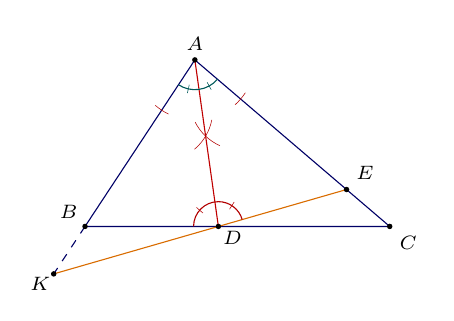
\begin{tikzpicture}[scale=0.90, every node/.style={font=\scriptsize}]
  \coordinate (A) at (0, 2.35);
  \coordinate (B) at (-1.55, 0);
  \coordinate (C) at (2.75, 0);
  \coordinate (D) at (0.3319, 0);
  \coordinate (E) at (2.1402, 0.5211);
  \coordinate (K) at (-1.9917,-0.6696);
  % ត្រីកោណ ABC និងបន្ទាត់បន្លាយ
  \draw[thin, blue!40!black] (A) -- (B) -- (C) -- cycle;
  \draw[thin, dashed, blue!40!black] (B) -- (K);
  \draw[thin, red!75!black] (A) -- (D);
  \draw[thin, orange!85!black] (E) -- (K);
  % ធ្នូមុំត្រង់ A (ពុះមុំ BAC: AB=-123.41, AD=-81.96, AC=-40.52)
  \draw[thin, teal!70!black] ($(A)+(-123.41:0.42)$) arc (-123.41:-40.52:0.42);
  \draw[very thin, teal!70!black] ($(A)+(-102.68:0.36)$) -- ($(A)+(-102.68:0.48)$);
  \draw[very thin, teal!70!black] ($(A)+(-61.24:0.36)$) -- ($(A)+(-61.24:0.48)$);
  % ធ្នូមុំត្រង់ D (ADB និង ADE: DB=180, DA=98.04, DE=16.08)
  \draw[thin, red!70!black] ($(D)+(180:0.35)$) arc (180:16.08:0.35);
  \draw[very thin, red!70!black] ($(D)+(139.02:0.29)$) -- ($(D)+(139.02:0.41)$);
  \draw[very thin, red!70!black] ($(D)+(57.06:0.29)$) -- ($(D)+(57.06:0.41)$);
  % ធ្នូសង់កន្លះបន្ទាត់ពុះមុំ AD (Compass construction arcs meeting on AD)
  \coordinate (P1) at ($(A)+(-123.4078:0.85)$);
  \coordinate (P2) at ($(A)+(-40.5154:0.85)$);
  \draw[very thin, red!70!black] ($(A)+(-131:0.85)$) arc (-131:-116:0.85);
  \draw[very thin, red!70!black] ($(A)+(-48:0.85)$) arc (-48:-33:0.85);
  \draw[very thin, red!70!black] ($(P1)+(-50:0.72)$) arc (-50:-11:0.72);
  \draw[very thin, red!70!black] ($(P2)+(-153:0.72)$) arc (-153:-114:0.72);
  % ចំណុចកំពូល
  \fill (A) circle (1.1pt) node[above] {$A$};
  \fill (B) circle (1.1pt) node[above left, inner sep=2.5pt] {$B$};
  \fill (C) circle (1.1pt) node[below right] {$C$};
  \fill (D) circle (1.1pt) node[below right, inner sep=1.5pt] {$D$};
  \fill (E) circle (1.1pt) node[above right] {$E$};
  \fill (K) circle (1.1pt) node[below left, inner sep=1pt] {$K$};
\end{tikzpicture}%
}
&
\par\vspace*{1.5cm}
\ditem បាទ/ចាស៎លោកគ្រូ \\
\end{longtable}

% -------------------- កាលបរិច្ឆេទ និងហត្ថលេខា (Date & Signature) --------------------
\vspace{6pt}
\hfill
\begin{minipage}{9.2cm}
  \centering
  ថ្ងៃពុធ ១១រោច ខែភទ្របទ ឆ្នាំមមី អដ្ឋស័ក ពុទ្ធសករាជ ២៥៧០\\[2pt]
  ត្រូវនឹងថ្ងៃទី៧ ខែតុលា ឆ្នាំ២០២៦\\[3pt]
  {\muol គ្រូបង្រៀន}\\[26pt]
  {\muol\hspace*{2.2cm}ហុក ប៊ុនថែន}
\end{minipage}

\end{document}
